  %%%%%%%%%%%%%%%%%%%%%%%%%%%%%%%%%%%%%%% -*- coding: utf-8; mode: latex -*- %%
  %
%%%%%                         CHAPTER
 %%%
  %

% $Id: 1020-lorem-ipsum.tex,v 1.2 2009/06/19 15:51:46 david Exp $
% $Log: 1020-lorem-ipsum.tex,v $
% Revision 1.2  2009/06/19 15:51:46  david
% *** empty log message ***
%
% Revision 1.1  2007/11/23 09:52:39  david
% *** empty log message ***
%
%

  %%%%%%%%%%%%%%%%%%%%%%%%%%%%%%%%%%%%%%%%%%%%%%%%%%%%%%%%%%%%%%%%%%%%%%%%%%%%%
  %
%%%%%                           HEAD MATTER
 %%%
  %

\chapter{Hadoop Open Platform as a service-HOP}
%\addcontentsline{lof}{chapter}{\thechapter\quad Lorem Ipsum}
%\addcontentsline{lot}{chapter}{\thechapter\quad Lorem Ipsum}
\label{ch:HOP}


  %%%%%%%%%%%%%%%%%%%%%%%%%%%%%%%%%%%%%%%%%%%%%%%%%%%%%%%%%%%%%%%%%%%%%%%%%%%%%
  %
%%%%%                        FIRST SECTION
 %%%
  %

\section{Introduction}

Hadoop Open Platform as a service (HOP) \cite{10} is a Hadoop distribution based
on Apache Hadoop . It provides namespace scalability through the support of multiple
NameNodes, platform as a service support for creating and managing clusters,
and a dashboard for simplified administration. HOP is developed in cooperation
of KTH and SICS \cite{15}


  %%%%%%%%%%%%%%%%%%%%%%%%%%%%%%%%%%%%%%%%%%%%%%%%%%%%%%%%%%%%%%%%%%%%%%%%%%%%%
  %
%%%%%                      SECOND SECTION
 %%%
  %

\section{HOP-HDFS}

HOP-HDFS\cite{11} \cite{12} is a fork of HDFS and part of HOP. It aims on providing high
availability and scalability for HDFS. This is achieved by making the NameNode
stateless and thereby adding support for the use of multiple NameNodes at the
same time. Instead of storing any state in the NameNode, the state is stored in
a distributed database offering high-availability and high-redundancy. Therefore,
the current implementation uses MySQL Cluster \cite{29}, which utilizes NDB Cluster
as an underlying storage engine.
HOP-HDFS is a promising approach that could make HDFS similar to Colos-sus, while overcoming the scalability and availability limitations of the current
Hadoop implementation. Through its support for larger amounts of metadata, it
could also make the use of block sizes smaller than 64 megabytes efficient, what
might be useful for many applications.



  %%%%%%%%%%%%%%%%%%%%%%%%%%%%%%%%%%%%%%%%%%%%%%%%%%%%%%%%%%%%%%%%%%%%%%%%%%%%%
  %
%%%%%                         ANOTHER SECTION
 %%%
  %
\subsection{HOP-HDFS Architecture}
The persistent data structures of HOP-HDFS (here after referred as HDFS) are defined as 11 database tables. These tables contain all the information about namespace,metadata,block locations and many other information that name-node in HDFS stores in FSImage and keeps in memory.
\begin{enumerate}
\item \textbf{inodes:} The  table  representing  inode  data  structure  in  HDFS  which  contains   the namespace  and  metadata  of  the  files   and  directories.  inodes   are  related  together  by their  parent\_ id  and  resembles   a  hierarchical  namespace  as   in  the  HDFS.  Each  row has a unique id which is the primary key.
\item \textbf{block\_ inofs:} Block   is   a  primitive  of  HDFS  storing  a  chunk   of  a  file,  block-info  is   its
metadata  keeping  a  reference  to  its   file-inode,  the  list  of  block’s   replica  which  are
scattered among multiple data-nodes.
\item \textbf{leases:} Basically   each  file  in  HDFS  is   either  underconstruction  or  completed.  All
underconstruction  files   are  assigned  a  sort  of  write  lock   to  them,  this   lock   is
persisted  in database. Each lease corresponds  to just one client machine, each client
could be writing multiple files at a time.

\item \textbf{lease\_ path:} Each  lease  path  represents   an  underconstruction  file, it holds  full path
of that file and points to the lease as its holder.

\item \textbf{replicas:} A  copy   of  a  Block   which  is   persisted  in  one  datanode,  sometime we refer
to replicas as blocks. All the replicas of the same block points to the same blockinfo.

\item \textbf{corrupted\_ replicas: }A replica become corrupted in the copy  operations  or due to the
storage  damages.  Namenode  realizes   this   by   comparing  checksum   in  the  report of
the replica’s datanode with the checksum of the original block.

\item \textbf{excess\_ replicas:} A  block   could  become  over replicated because of an already  dead
datanode  coming  alive  again  and  contain  some  replicas   which  has   been  removed
meanwhile  from   namenode.  So  distinguishing  that,  namenode  marks   marks   some
replicas to be removed later on.

\item \textbf{invalidated\_ blocks:} For  every   datanode  keeps   a  list  of  blocks   that  are  going  to  be
invalidated(removed) on that datanode due to any reason.

\item \textbf{replicas\_ under\_ construction:} Replications   of  a  block   which  are  being  streamed  by
client into datanodes.

\item \textbf{under\_ replicated\_ blocks:} Keeps   track   of  the  blocks   which  has   been  under
replicated,  it  realizes   the  priority   of  under  replications   as   follow.  Priority   0  is   the
highest  priority.  Blocks   having  only   one  replica  or  having  only   decommissioned
replicas   are  assigned  priority   0.  Blocks   having  expected  number  of  replicas   but  not
enough  racks   are  assigned  with  priority   3.  If  the  number  of  replicas   of  a  block   are  3
times   less   than  expected  number  of  replicas   then  the  priority   is   assigned  to  1.  The
rest  of  low  replication  cases   are  assigned  priority   2.  Blocks   having  zero  number  of
replicas   but  also  zero  number  of  decommissioned replicas  are assigned priority  4 as
corrupted blocks.

\item \textbf{pending\_ blocks:} Represents a blocks that are being replicated.

\end{enumerate}
 The figure \ref{fig:HDFS_table_relation} illustrates the relation between tables. The figure \ref{fig:HDFS_table_schema} gives the columns stored in each table.
\begin{figure}[h!]
  \centering
 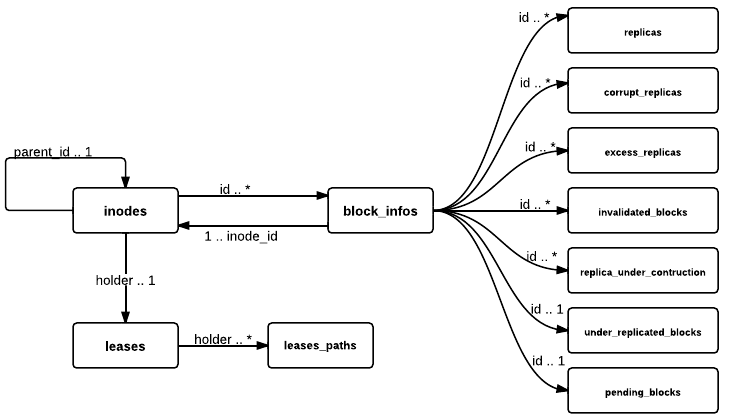
\includegraphics[scale=0.5]{figs/preliminar/HOP_table_relation.png}
  \caption{HOP-HDFS Table relations.}
  \label{fig:HDFS_table_relation}
\end{figure}
\pagebreak
\begin{figure}[h!]
  \centering
 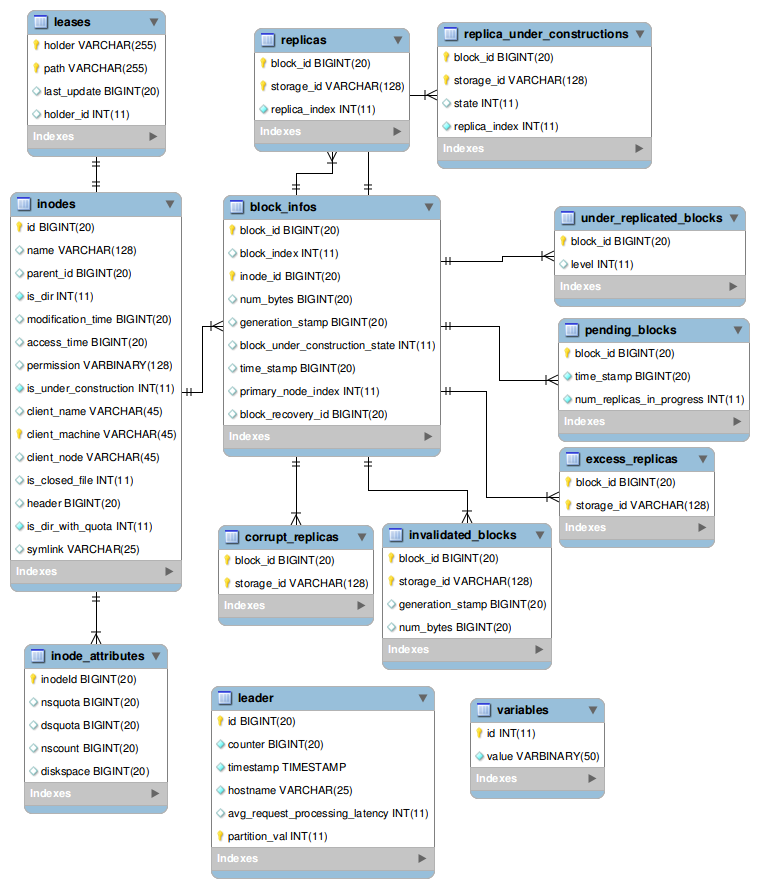
\includegraphics[scale=0.5]{figs/preliminar/HOP_HDFS_Schema.png}
  \caption{HOP-HDFS Schema}
  \label{fig:HDFS_table_schema}
\end{figure}



  %%%%%%%%%%%%%%%%%%%%%%%%%%%%%%%%%%%%%%%%%%%%%%%%%%%%%%%%%%%%%%%%%%%%%%%%%%%%%
  %
%%%%%                          LAST SECTION
 %%%
  %

\subsection{NameNode Operations}

Every   operation  defined  in  the  HDFS  client  API  (such  as   createFile,  open,  etc)  maps   onto  one  or  more  of  the  following  primitive  HDFS  operations.  Each  operation  defined  in  the primitive  HDFS  API  maps  onto a protocol message (where each protocol message contains request, reply, and exception  parts) sent between the NameNode, client, and DataNodes. Some  common   primitive  operations  are  shown   in   the  table \ref{NameNode_Ops}.  The  full  list  of  the primitive operations can be found in Thesis report \cite{12} Appendix section.
\begin{table}[t]
\centering
\begin{tabular}{|l|p{12cm}|}
\hline
\textbf{OPERATION} & \textbf{SUMMARY}\\
\hline
\textbf{MKDIR}&Creates   a  directory   recursively,  it  requires   a  no
lock   on  all  the  existing  components   of  the  path
but  write  lock   on  the  last existing.\\
\hline
\textbf{START\_ FILE} & \begin{enumerate}
\item If  file  does   not  exist,  It  creates   inodes
for  all  the  nonexistent  directories   and
new  file,  writes   owner  of  the  lease  and
creates new leasepath.
\item If  file  already   exists   first  removes   the
file,  its   blocks   and  dependencies,  lease
and  lease  path,  then  it  does   the  first
scenario.
\end{enumerate}\\
\hline
\textbf{GET\_ ADDITIONAL\_ BLOCK}&  In  the  middle  of  writing  a  file,  this   is   the  client’s
           mean  of  noticing  namenode  that  the  already
                 being  written  block   is   finished  while  it  is   asking
                        for  the  locations   of  next  block.  NameNode
                             removes   all  the  replicaunderconstructions   of
                                  last  block, it also changes  type of blockinfo from
                                          underconstruction  to  completed  one.\\

\hline
\textbf{COMPLETE}& Like  get\_ additional\_ block,  it  happens   for  last
    block   of  the  file,  NameNode  just  removes   the
          replicaunderconstructions   and  changes   type  of
               blockinfo from underconstruction to completed.
 \\
\hline
\textbf{GET\_ BLOCK\_ LOCATIONS}& Given  path  of  the  file,  it  returns   location  if  its
        blocks and updates accesstime of the fileinode.
 \\ 
 \hline
 \textbf{DELETE} & Delete the given file or directory from the file system.\\
 \hline
 \textbf{RENAME} & Renames gives SRC to DST. Without OVERWRITE option, rename fails if the dst already exists. With OVERWRITE option, rename overwrites the dst, if it is a file 
    or an empty directory. Rename fails if dst is a non-empty directory. The rename opeartion is atomic.\\
\hline 
 \textbf{APPEND} & Append to the end of the file.It retuns the partially completed last block if any. \\
 \hline
\end{tabular}
\caption{NameNode's Operations}
\label{NameNode_Ops}
\end{table}

\subsection{HOP-HDFS Implementation}
n HOP-HDFS each HDFS opeartion is implemented as a single transaction,where after transaction began, read and write the necessary meta-data from NDB , and then either commit the transaction, or in case of failure, the transaction was aborted and then possibly retried. However,  the  default  isolation  level  of  NDB  is   read  committed,  which  allows   the  results   of
write  operations   in  transactions   to  be  exposed  to  read  operations   in  different  concurrent
transactions.  This   means   that  a  relatively   long  running  read  transaction  could  read  two
different  versions   of  data  within  the  same  transaction,  known  as  a fuzzy  read, or it could get
different  sets   of  results   if the same query  is  issued twice within the same transaction  this  is
known as a phantom read. In report\cite{12} and paper \cite{hoppaper} they proposed and implemented the snapshot-isolation method \ref{hopAlgo} which pessimistically locks the rows of data preventing other transactions from accessing. 

\begin{algorithm}[h]
\caption{Snapshotting taking locks in a total order}
\label{hopAlgo}
\begin{algorithmic}

\State snapshot.clear \\ \\

\textbf{Operation } doOperation \\

\State tx.begin
\State create-snapshot()
\State performTask()
\State tx.commit\\

\State \textbf{Operation} create-snapshot \\
\State S = total\_ order\_ sort(op.X) 
\ForAll{x in S}
\If{x is a parent }
\State level = x.parent\_ level\_ lock
\Else
\State level = x.strongest\_ lock\_ type
\State tx.lockLevel(level)
\State snapshot $<$- tx.find(x.query)
\EndIf
\EndFor
 \\ 
\State \textbf{Operation} performTask
\State //Operation Body,referring to transaction cache for data

\end{algorithmic}
\end{algorithm}

\section{MySQL Cluster}
Mysql  Cluster  is   a  Database  Management  System   (DBMS)  that  integrates   the  standard
Mysql  Server with an inmemory  clustered storage engine called NDB Cluster (which stands
for  “Network   DataBase”)  .  It  provides   a  sharednothing  system   with  no  single
point of failure.

\begin{figure}[hb]
\centering  
 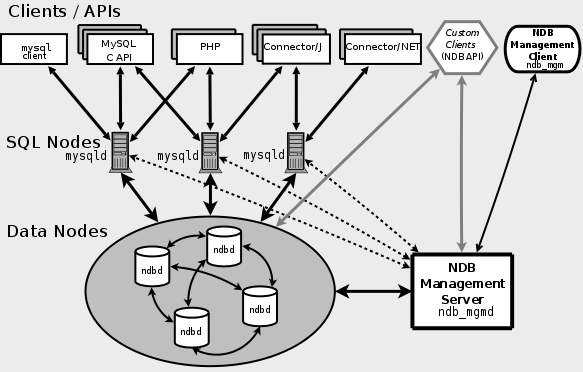
\includegraphics[scale=0.75]{figs/preliminar/mysql_cluster.png}
  \caption{MySQL cluster}
  \label{fig:mysqlCluster}
\end{figure}


Mysql  Cluster  is   a  compound  of  different  processes   called  \textbf{nodes}.  The  main  nodes   are
Mysql  Servers   (mysqld,  for  accessing  NDB  data),  data  nodes   (ndbd,  as   the  data  storage),
one  or  more  management  servers   (ndb\_ mgmd).  The  relationship  between  these  nodes   are
shown in figure \ref{fig:mysqlCluster}.
The  data  in Mysql Cluster is  replicated over multiple ndbds  so this  makes  the database to be
available  in  case  of  node  failures.  Ndbds   are  divided  into \textbf{node groups}.  Each  unit  of  data
stored  by   ndbd  is   called  a  \textbf{partition}.  The  partitions   of  data  are  replicated  into  ndbds   of  the
same node group while node groups are calculated indirectly as following:
$$Number of Node groups  = \frac{number of  datanodes}{number of  replicas} $$
A  simple  cluster  of  4  datanodes   with  replication  factor  of  2  and  consequently  2 node groups
are shown in figure 8.
As   it  can  be  seen,  the  data stored in the database are divided into 4 partitions. There are two
replicas   of  each  partition  into  ndbds   of  the  same  node  group.  So  even  if  one  of the ndbds  in
each  of  the  node  groups   are  failed, the whole data in the cluster will be available. However, if
both  ndbs   in a node group become unavailable then those partitions  stored by  the failed ndbs
also will become unavailable.
According  to  a  white  paper  published  by   Oracle  ,  Mysql  Cluster  can  handle  4.3
billion  fully   consistent  reads   and  1.2  fully  transactional writes  per minute. They  used an open
source  benchmark   called  flexAsynch  and  a  Mysql  Cluster  of  30  data  nodes,  comprised  15
node  groups.  The  detail  of  their  system   configuration  is   available  in  the  referenced  white
paper. The results for write operations are shown in figure \ref{fig:mysqlCluster}.
The  72  million  reads   and  19.5  million  write  operations   per  second  of  Mysql  Cluster  shows
that it has a high throughput for simple read and write operations.

\subsection{Concurrency Control in NDBCluster}
NDB  supports   pessimistic   concurrency   control  based  on  locking.  It  supports   row  level
locking.  NDB  throws   a timeout error if a requested lock  cannot be acquired within a specified
time \cite{mysql1}.  Concurrent  transactions,  requested  by   parallel  threads   or  applications,
reaching  the  same  row  could  end  up  with  deadlock.  So,  it  is   up  to  applications   to  handle
deadlocks   gracefully.  This   means   that  the  timed  out  transaction  should  be  rolled  back   and
restarted.  Transactions   in  NDB  are  expected  to  complete  within  a  short  period  of  time,  by
default  2  seconds.  This   enables   NDB  to  support  realtime  services,  that  are,  operations
expected  to  complete  in  bounded  time.  As   such,  NDB  enables   the  construction  of  services
that  can  failover,  on  node  failures,  within  a  few  seconds     ongoing transactions  on the node
that  dies  timeout within a couple of seconds, and its  transactions  can be restarted on another
node in the system.

\subsection{ClusterJ}
Clusterj  is   Java  connector  implementation  of  NDB  Cluster,  Mysql  Cluster’s   storage  engine, \cite{29}.  Clusterj  uses   a  JNI  bridge  to  the  NDB  API  to  have  a  direct  access   to  NDB
Cluster.  The  NDB  API  is   an  application  programming  interface  for  Mysql  Cluster  that
implements   indexes,  scans,  transactions   and  event  handling.  Clusterj  connects   directly   to
NDB  Clusters   instead  of  connecting  to  mysqld.  It  is   a  persistence  framework   in  the  style of
Java  Persistence  API.  It  provides   a  data  mapper  mapping  java  classes   to  database  tables
which separates the data from business logic.

  %
 %%%
%%%%%                        THE END
  %
  %%%%%%%%%%%%%%%%%%%%%%%%%%%%%%%%%%%%%%%%%%%%%%%%%%%%%%%%%%%%%%%%%%%%%%%%%%%%%

%%% Local Variables: 
%%% mode: latex
%%% TeX-master: "tese"
%%% End: 
